\chapter{Price of connectivity for vertex cover}\label{chap3}
\begin{thm}\label{pocVC:1}
For every graph \(G\) with at least one edge it holds that \( 1 \leq \frac{\tau_c(G)}{\tau(G)} < 2\).
\end{thm}
\begin{myproof}
	Let \(C\) be any vertex cover of a connected graph \(G\) and \(c\) the number of components of \(G[C]\).
	Then we can add at most \(c - 1\) vertices to \(C\) to construct a connected vertex cover of \(G\).
	Thus \(\tau_c(G) \leq {2\tau(G) - 1}\).
	The size of a minimum connected vertex cover is at least the size of a minimum vertex cover.
	For the ratio \(\frac{\tau_c(G)}{\tau(G)}\) to be defined \(G\) must contain at least one edge, 
	otherwise both numbers \(\tau\) and \(\tau_c\) are equal to zero.
\end{myproof}

Example of graphs for which \(\tau_c(G)= 2\tau(G) - 1\) holds are odd length paths and cycles with an even number of vertices.
For this class of graphs we can say, that the upper bound from the previous theorem is asymptotically sharp because:

\[\lim_{k \to \infty}{\frac{\tau_c(G)}{\tau(G)}} = \lim_{k \to \infty}{\frac{2k - 1}{k}} = 2.\]

Earlier we discussed that deciding whether the price of connectivity for a graph \(G\) is bounded by a number \(t \in (1, 2)\) is \(\Theta^p_2\)-complete.
One can ask how to weaken this problem as little as possible to make it polynomially solvable.
Let us focus on classes of graphs for which the number \(\frac{\tau_c(G)}{\tau(G)}\) is bounded by a fixed number \(t\) for every induced subgraph of \(G\).
Classes which are closed under induced subgraphs are called hereditary.

Camby et al. in \cite{CambyCardinalFioriniSchaudt14} characterize hereditary graph classes with PoC upper-bounded by \(1\), \(\frac{4}{3}\) and \(\frac{3}{2}\).
%%In \cite{Camby19} Camby later proposed a conjecture how to characterize hereditary classes with PoC at most \(\frac{5}{3}\).
All these classes were determined by a finite list of forbidden induced subgraphs.
Such characterization gives us a polynomial time recognition algorithm.
For a given graph \(G\) and every graph \(H_i\) from the list of forbidden subraphs it is enough to check each vertex subset of \(G\) with the size \(|V(H_i)|\)
if it induces graph \(H_i\). The length of the list is finite and independent from the size of \(G\) and the number of all checked subsets is polynomial in the number of vertices
in \(G\).

The following two sections \ref{3:1} and \ref{3:2} are devoted to the characterization of hereditary classes given in \cite{CambyCardinalFioriniSchaudt14}.   
\section{PoC-perfect graphs for vertex cover}\label{3:1}
\begin{defn}
A graph \(G\) is called \emph{PoC-perfect} if every subgraph \(H\) of \(G\) satisfies \(\tau_c(H)=\tau(H)\).
\end{defn}

Class of PoC-perfect graphs is described in this theorem.
\begin{thm}[\citet{CambyCardinalFioriniSchaudt14}]\label{pocVC:1}
The following assertions are equivalent for every graph \(G\) :
\begin{itemize}
\item For every induced subgraph \(H\) of \(G\) it holds that \(\tau_c(H) = \tau (H)\).
\item \(G\) is \((P_5, C_5, C_4)\)-free.
\item \(G\) is chordal and \(P_5\)-free.
\end{itemize}
\end{thm}

It is easy to observe that \(\tau(C_4) = \tau(P_5) = 2\) and \(\tau_c(C_4) = \tau_c(P_5) = 3\).
The price of connectivity of \(C_5\) is \(\frac{4}{3}\). 
Since these graphs are not PoC-perfect then they cannot be induced subgraphs of PoC-perfect graphs.

\section{PoC-near-perfect graphs for vertex cover}\label{3:2}

\begin{defn}
A graph \(G\) is \emph{PoC-near-perfect} with a threshold \(t \in (1, 2)\) if every subgraph \(H\) of \(G\) satisfies the inequality \(\frac{\tau_c(H)}{\tau(H)} \leq t\).
\end{defn}

\begin{thm}[\citep{CambyCardinalFioriniSchaudt14}]\label{pocVC:2}
The following assertions are equivalent for every graph \(G\) :
\begin{itemize} 
\item For every induced subgraph \(H\) of \(G\) it holds that \(\tau_c(H) \leq {\frac{4}{3} \tau(H)}\).
\item \(G\) is \((P_5 , C_4)\)-free.
\end{itemize}
\end{thm}

\begin{thm}[\citep{CambyCardinalFioriniSchaudt14}]\label{pocVC:3}
The following assertions are equivalent for every graph \(G\):
\begin{itemize}
\item For every induced subgraph \(H\) of \(G\) it holds that \(\tau_c(H) \leq \frac{3}{2}\tau(H)\).
\item \(G\) is \((P_7 , C_6 , \Delta_1 , \Delta_2)\)-free.
\end{itemize}
\end{thm}

The graph \(\Delta_1\) is constructed from two disjoint copies of \(C_4\) by identifying two vertices each from a different copy of \(C_4\).
\(\Delta_2\) is obtained from \(\Delta_1\) by deleting an edge incident to a vertex with degree four. 
For illustration see the Figure~\ref{pic:deltas}.
%%Insert Pictures of Deltas
\begin{figure}[b]
        \centering
        \begin{minipage}{.5\textwidth}
                \centering
                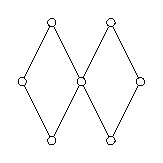
\includegraphics[width=.5\linewidth]{pictures/VCpocdelta1}
		\caption*{}
        \end{minipage}%
        \begin{minipage}{.5\textwidth}
                \centering
                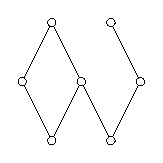
\includegraphics[width=.5\linewidth]{pictures/VCpocdelta2}
                \caption*{}
        \end{minipage}
        \caption{Graphs $\Delta_1$ and $\Delta_2$ from Theorem~\ref{pocVC:3}.}
	\label{pic:deltas}
\end{figure}
%%
%%
%%ToDo Only proof sketch of Theorem~\ref{pocVC:2}
%%
We will present two lemmata which are used in proofs of Theorem~\ref{pocVC:2} and Theorem~\ref{pocVC:3}.
These structural properties may be useful while trying to derive similar results for different values of the parameter \(t\).

\begin{lemma}[\citet{CambyCardinalFioriniSchaudt14}]
Let \(G\) be a connected graph and let \(C\) be a vertex cover of \(G\). 
Suppose	that \((\mathcal{A}, \mathcal{B})\) is a bipartition of the connected components of \(C\) with \(\mathcal{A}, \mathcal{B} \neq \emptyset\), then there
exist two components \(A\) and \(B\) each from different parts such that the number of vertices on the shortest path from \(A\) to \(B\) is 3.
\end{lemma}

\begin{myproof}
	Let us pick two components \(A \in \mathcal{A}\) and \(B \in \mathcal{B}\) with the minimum distance. 
	Such pair exists because \(C\) has a finite number of connected components.
	Path \(x_1, \dots, x_k\) is the shortest path between \(A\) and \(B\). Vertex \(x_1 \in A\) and \(x_k \in B\).
	On the contrary we suppose that \(k > 3\). 
	None of the vertices \(x_2, \dots x_{k-1}\) belong to \(C\). Otherwise, \(B\) is not the nearest component to \(A\).
	Edge \(x_2, x_3\) is not covered, but that contradicts that \(C\) is a vertex cover.
\end{myproof}

Let \(C\) be a vertex cover of a connected graph \(G\) and \(S\) be a connected component of \(C\).
Then \(P_C(S)\) denotes a set of vertices \(v \in V(G)\) such that \(N(v) \cap C \subseteq V(S)\).
In other words, \(P_C(S)\) contains \(S\) and vertices whose entire neighborhood is in \(S\).
In particular \(P_C(S)\) induces connected subgraph in \(G\).
\begin{lemma}[\citet{CambyCardinalFioriniSchaudt14}]
Let \(S_1, S_2, \dots, S_k\) be connected components of a
vertex cover \(C\). There exists at least one \(P_C(S_i)\) which is not a cutset of \(G\), i.e.
\(G[V(G) \setminus P_C(S_i)]\) is connected.
\end{lemma}

\begin{myproof}
	Sets \(P_C(S_i)\) are disjoint by definition.
	We define a new graph \(H\) with vertices corresponding to the sets \(P_C(S_i)\).
	Two vertices \(P_C(S_i)\) and \(P_C(S_j)\) are adjacent in \(H\) if neighborhoods of \(P_C(S_i)\) and \(P_C(S_j)\) 
	share at least one vertex.
	Formally:
	 \[V(H) = \{P_C(S_i): i \in \{1, \dots, k\}\}\]
	 and
	 \[E(H) = \{P_C(S_i), P_C(S_j)|  P_C(S_i) \cap P_C(S_j) \neq \emptyset\}.\]
	Since \(G\) is connected and \(C\) is a vertex cover, graph \(H\) is connected.
	Every connected graph contains at least one vertex that is not a cut vertex.
	Thus, in \(G\) there exists a set \(P_C(S_i)\) that is not a cutset. 
\end{myproof}

\section{PoC critical graphs for vertex cover}

\begin{defn}
A graph \(G\) is \emph{critical} if every induced subgraph \(H\) of \(G\) has strictly smaller price of connectivity than \(G\).
\end{defn}

Critical graphs are precisely those which can be listed in forbidden subgraphs characterization. Note that all previous examples of forbidden subgraphs are also critical.
In this section we will investigate structure of critical graphs in more detail.

Many proofs from this section will use the following inequality to derive a contradiction.

\begin{lemma}\label{VC:fracsum}
	Let \(\frac{a_1}{b_1}, \dots, \frac{a_i}{b_i}, \dots \frac{a_n}{b_n}\) be real fractions with positive denominator.
	Denote the largest and the smallest fraction \(M\) and \(m\) respectively.
	Then \[{m} \leq {\frac{\sum_{i=1}^{n}{a_i}}{\sum_{i=1}^{n}{b_i}}} \leq {M}\].
\end{lemma}

\begin{myproof}
	We observe that the following iquality holds:
	\[{a_1 + a_2 + \dots + a_n} = {b_1 q_1 + b_2 q_2 + \dots + b_n q_n},\] 
	where \(q_i\) is equal to \(\frac{a_i}{b_i}\).
	The expression on the right is clearly at most \((b_1 + \dots + b_n)M\) and at least \((b_1 + \dots + b_n)m\).
	To finish the proof it is enough to divide both sides of the inequality by the sum \(b_1 + \dots + b_n\).
\end{myproof}

\begin{lemma}[\citet{CambyCardinalFioriniSchaudt14}]\label{VC:Bridge}
Let \(G\) be a critical graph. An edge with both endpoints in the minimum size vertex cover cannot be a bridge in \(G\).
\end{lemma}
\begin{myproof}
	Suppose for the sake of contradiction that \(G\) has a minimum vertex cover with vertices \(x\), \(y\), such that edge \(xy\) is a bridge.
	This means that graph \(G \setminus (xy)\) has two connected components \(C_1\) and \(C_2\).
	\(C_1\) is adjacent only to \(x\) and \(C_2\) is adjacent only to \(y\).
	Consider two induced subgraphs \(H_1\) and \(H_2\) defined like this.
	The subgraph \(H_i\) contains \(C_i\) and vertices \(x\) and \(y\).
	The minimum vertex cover of \(G\) must have at least \(\tau(H_1) + \tau(H_2)\) vertices, because both vertices \(x\) and \(y\)  %%Vysvetlit lepe
	are in the minimum vertex cover of \(G\) and components \(C_1\) and \(C_2\) are disjoint.
	On the other hand, union of connected vertex covers of \(H_1\) and \(H_2\) is also a connected vertex cover of \(G\) because vertices \(x\), \(y\) are in the union
	and edge \(xy\) is a bridge.
	So number \(\tau_c(G)\) is at most \(\tau_c(H_1) + \tau_c(H_1)\).
	These inequalities together with Lemma~\ref{VC:fracsum} yields:
	\[{\frac{\tau(G)}{\tau_c(G)}} \leq {\frac{\tau(H_1) + \tau(H_2)}{\tau_c(H_1) + \tau_c(H_2)}} \leq {\max\left\{\frac{\tau(H_1)}{\tau_c(H_1)}, \frac{\tau(H_2)}{\tau_c(H_2)}\right\}}\]
	That contradicts the assumption that \(G\) is critical.
\end{myproof}

The technique demonstrated above allows us to derive further structural results about critical graphs.

\begin{lemma}\label{VC:IndNeig}
Let \(G\) be a critical graph, let a vertex \(x\) be an arbitrary vertex from a minimum size vertex cover. Then \(N(x)\) is an independent set.
\end{lemma}

%%Illustration of case on proof of Lemma~\ref{VC:IndNeig}
\begin{figure}
        \centering
        \begin{minipage}{.45\textwidth}
                \centering
                \def\offset{2}
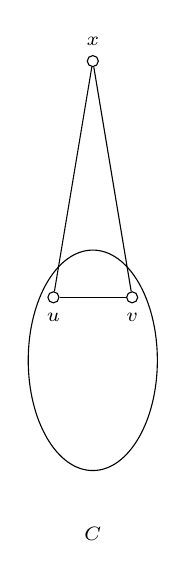
\begin{tikzpicture}

                \tikzstyle{vertex}  = [circle, minimum width=4pt, draw, inner sep=0pt, fill=white]
                \node [vertex, label=above:{\scriptsize$x$},](x) at (2.5, 6) {};
                \node [vertex, label=below:{\scriptsize$u$}](u) at ({0 + \offset}, 3) {};
                \node [vertex, label=below:{\scriptsize$v$}](v) at ({1 + \offset}, 3) {};
                \draw ({0 + \offset + 0.5}, 2.2) ellipse (0.82cm and 1.4cm);
                \node (c) at ({0 + \offset + 0.5}, 0) {\scriptsize$C$};
                \draw (u) -- (v);
                \draw (u) -- (x);
                \draw (v) -- (x);
\end{tikzpicture}


                \caption*{First case}
        \end{minipage}%
        \begin{minipage}{.45\textwidth}
                \centering
                \def\offset{2}
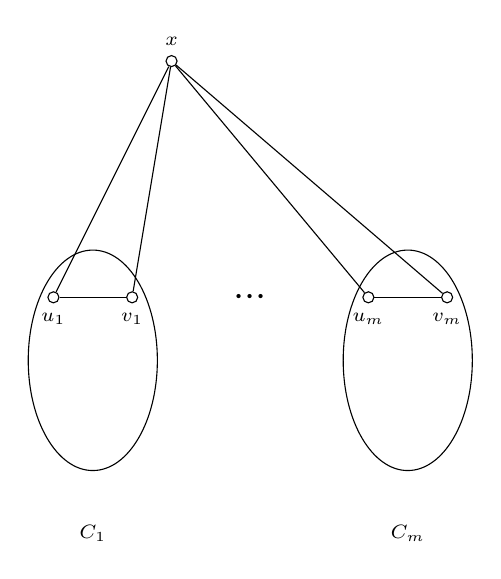
\begin{tikzpicture}

                \tikzstyle{vertex}  = [circle, minimum width=4pt, draw, inner sep=0pt, fill=white]
                \node [vertex, label=above:{\scriptsize$x$},](x) at (3.5, 6) {};

                \foreach \i in {1,2}
                {
                        \ifnum \i = 2
                                \node [vertex, label=below:{\scriptsize$u_m$}](u\i) at ({2 + \i * \offset}, 3) {};
                                \node [vertex, label=below:{\scriptsize$v_m$}](v\i) at ({3 + \i * \offset}, 3) {};
                                \node [minimum size=2.5cm, minimum width = 7pt](dots) at ({((2 + \i * \offset) - ( 1 + (\i-1) * \offset))*0.5 + ((1 + (\i-1) * \offset))}, 3) {\huge{$\scriptstyle \cdots$}};

                                \draw ({2 + \i * \offset + 0.5}, 2.2) ellipse (0.82cm and 1.4cm);
                                \node (c\i) at ({2 + \i * \offset + 0.5}, 0) {\scriptsize$C_m$};



                        \else
                                \node [vertex, label=below:{\scriptsize$u_\i$}](u\i) at ({0 + \i * \offset}, 3) {};
                                \node [vertex, label=below:{\scriptsize$v_\i$}](v\i) at ({1 + \i * \offset}, 3) {};
                                \draw ({0 + \i * \offset + 0.5}, 2.2) ellipse (0.82cm and 1.4cm);
                                \node (c\i) at ({0 + \i * \offset + 0.5}, 0) {\scriptsize$C_\i$};


                        \fi

                        \draw (u\i) -- (v\i);
                        \draw (u\i) -- (x);
                        \draw (v\i) -- (x);


                }

\end{tikzpicture}


                \caption*{Second case}
        \end{minipage}
	\hfill
	\begin{minipage}{.45\textwidth}
                \centering
                \def\offset{2}
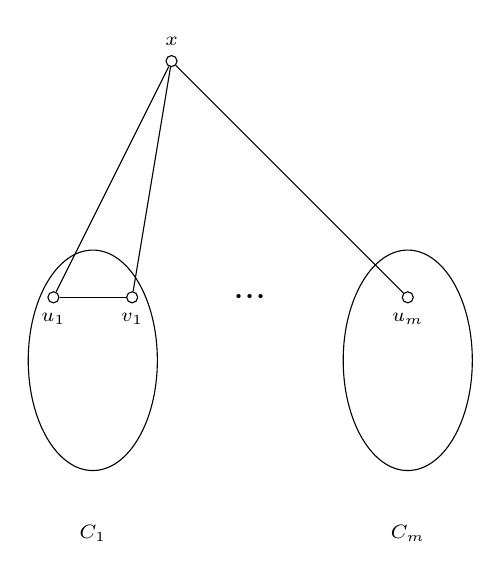
\begin{tikzpicture}
        \tikzstyle{vertex}  = [circle, minimum width=4pt, draw, inner sep=0pt, fill=white]
                \node [vertex, label=above:{\scriptsize$x$},](x) at (3.5, 6) {};

                \foreach \i in {1,2}
                {
                        \ifnum \i = 2
                                \node [vertex, label=below:{\scriptsize$u_m$}](u\i) at ({2.5 + \i * \offset}, 3) {};
                                \node [minimum size=2.5cm, minimum width = 7pt](dots) at
                                ({((2 + \i * \offset) - ( 1 + (\i-1) * \offset))*0.5 + ((1 + (\i-1) * \offset))}, 3) {\huge{$\scriptstyle \cdots$}};

                                \draw ({2 + \i * \offset + 0.5}, 2.2) ellipse (0.82cm and 1.4cm);
                                \node (c\i) at ({2 + \i * \offset + 0.5}, 0) {\scriptsize$C_m$};
                                \draw (u\i) -- (x);
                        \else
                                \node [vertex, label=below:{\scriptsize$u_\i$}](u\i) at ({0 + \i * \offset}, 3) {};
                                \node [vertex, label=below:{\scriptsize$v_\i$}](v\i) at ({1 + \i * \offset}, 3) {};
                                \draw ({0 + \i * \offset + 0.5}, 2.2) ellipse (0.82cm and 1.4cm);
                                \node (c\i) at ({0 + \i * \offset + 0.5}, 0) {\scriptsize$C_\i$};
                                \draw (u\i) -- (v\i);
                                \draw (u\i) -- (x);
                                \draw (v\i) -- (x);
                        \fi
                }
\end{tikzpicture}


                \caption*{Third case}
        \end{minipage}

	\caption{Illustration of the cases from the proof of Lemma~\ref{VC:IndNeig}.}
\end{figure}
\begin{proof}[Proof of Lemma \ref{VC:IndNeig}]
Let \(G\) be a critical graph and \(S\) a minimum vertex cover of \(G\) and vertex \(x \in S\).
For the sake of contradiction suppose there are two adjacent vertices \(u\) and \(v\) in \(G\) such that \(u, v \in N(x)\).
We will distinguish between these three cases.
\begin{enumerate}
\item The vertex \(x\) is not a cut vertex.
	
	Let \(H\) be the graph obtained by deleting of \(x\).
	Clearly \(\tau(G)\) is at most \(\tau(H) + 1\) because minimum vertex cover of \(H\) together with vertex \(x\) is a vertex cover of \(G\).
	The opposite inequality is also true. Notice that \(S \cap V(H)\) is a minimum vertex cover of \(H\). 
	A minimum connected vertex cover of \(H\) together with vertex \(x\) is also a connected vertex cover of \(G\).
	That is true because any vertex cover of \(H\) must include at least one vertex from the edge \(uv\) and both vertices are neighbors of \(x\). 
	Thus, \(\tau_c(G)\) can be bounded from above by this expression:
        	\[\tau_c(G) \leq {\tau_c(H}) + 1.\]
	Using these two inequalities and inequality from Lemma~\ref{VC:fracsum} gives us:	
		\[{\frac{\tau_c(G)}{\tau(G)}} \leq {\frac{\tau_c(H) + 1}{\tau(H) + 1}} \leq {\max\left\{ \frac{\tau_c(H)}{\tau(H)}, 1\right\}}.\]
	
	For every graph \(G\) the ratio between \(\tau\) and \(\tau_c\) is at least one.
	That means that the induced subgraph \(H\) of \(G\) satisfies \(\frac{\tau_c(G)}{\tau(G)} \leq {\frac {\tau_c(H)}{\tau(H)}}\).
	However, that contradicts the criticality of \(G\).
	
\item The vertex \(x\) is a cut vertex and each component in the graph \(G \setminus \{x\}\) has an edge in \(N(x)\).
	
	Denote these components \(C_1, C_2, \dots, C_m\).
	\begin{claim}
		\(\tau(G) = {\sum_{i = 1}^{m}{\tau(C_i)} + 1}\)
	\end{claim}
	The inequality \(\tau(G) \leq {\sum_{i = 1}^{m}{\tau(C_i)} + 1}\) is easy to see as the union of minimum vertex covers of \(C_i\) with vertex \(x\) is a vertex cover of the entire graph.
	
	Observe that \(S \cap V(C_i)\) is also a minimum vertex cover of \(C_i\). This implies the desired inequality.
		\[\tau(G) \geq {\sum_{i=1}^{m}{\tau(C_i)} + 1}.\]
	The claim is proved.
	
	We need to find an upper bound for a size of a minimum connected vertex cover of \(G\).
	The union of minimum connected vertex covers of \(C_i\) and vertex \(x\) make a connected vertex cover of \(G\).
	The reason is that each vertex cover of \(C_i\) contains at least one neighbor of \(x\) due to edges in \(V(C_i) \cap N(x)\).
	This yields the following upper bound:
		\[\tau_c(G) \leq {\sum_{i=1}^{m}{\tau_c(C_i)} + 1}.\]
	Let us combine all estimates together and then use Lemma~\ref{VC:fracsum}:

	\[\frac{\tau_c(G)}{\tau(G)} \leq {\frac{\tau_c(C_1) +, \dots, + \tau_c(C_m) + 1}{\tau(C_1) +,\dots, + \tau(C_m) + 1}} 
	\leq \max\left\{ \frac{\tau_c(C_i)}{\tau(C_i)}, 1\right\}.\]

	Again we have a contradiction with the assumption that \(G\) is critical.	

\item 
	The vertex \(x\) is a cut vertex and at least one component in \(G \setminus \{x\}\) does not have an edge in \(N(x)\).

	Additionally, we can assume that in \(G\) there is one component \(C_1\) with an edge \(uv\) in \(N(x)\). 
	The proof is complete otherwise.
	We denote such components \(C_1, \dots, C_m\).
	Consider all these induced subgraphs of \(G\): \(H_1\), \(C_1\), \dots, \(C_m\).
	Subgraph \(H_1\) includes all components without an edge in \(N(u)\) together with vertices \(x\) and \(u\).
	Without loss of generality we can assume that \(x\) is in some minimum vertex cover of \(H_1\). If it is not that the case that we know that in the minimum vertex cover is \(v\).
	We can switch \(v\) with vertex \(x\). Again this is a vertex cover of \(H_1\) because \(v\) is a leaf in \(H_1\).
	That implies that union of minimum vertex covers of \(H_1\) and \(C_i\) is a vertex cover of \(G\). 
	Conversely the size of minimum vertex cover of \(G\) is at least \(\tau(H_1) + \tau(C_1), + \dots, \tau(C_m)\).
	\(D \cap C_i\) is vertex cover of \(C_i\) and \(x\) is already counted in \(\tau(H_1)\).
	Observe that vertex \(x\) must be in any connected vertex cover of \(H_1\) because an edge \(xv\) needs to be covered and \(x\) is a cut vertex in \(H_1\).
	Also leaf \(v\) is not in any minimum connected vertex cover of \(H_1\). That means that in the sum of \(\tau_c\) of our subgraphs vertices \(x\) and \(v\)
	are counted no more than once.
	Using this and inequality from Lemma~\ref{VC:fracsum} we can estimate the ratio between \(\tau(G)\) and \(\tau_c(G)\) in the following way:	
	
	\[\frac{\tau_c(G)}{\tau(G)} \leq {\frac{\tau_c(H_1) + \tau_c(C_1) +, \dots, \tau(C_m)}{\tau(H_1) + \tau(C_1), + \dots, \tau(C_m) }} \leq 
	{\max\left\{ \frac{\tau_c(H_1)}{\tau(H_1)}, \frac{\tau_c(C_i)}{\tau(C_i)}\right\}}.\]

	This inequality implies that for one of the induced subgraphs \(H_1\) or \(C_i\) their price of connectivity is at least equal to \(\frac{\tau_c(G)}{\tau(G)}\), 
	but that contradicts assumption about criticality of \(G\). 
\end{enumerate}
\leavevmode
\end{proof}

\begin{lemma}\label{VC:1compNoEdge}
	Let \(G\) be a critical graph with \(\frac{\tau_c(G)}{\tau(G)} \geq \frac{3}{2}\) and 
	a minimum vertex cover contains two vertices \(x\), \(y\) such that \(G \setminus \{x, y\}\) is connected.
	Then \(N(x) \cup N(y)\) is an independent set. In particular \(xy \not\in E\).
\end{lemma}

\begin{myproof}
	Suppose that there is an edge between two vertices \(u \in N(x)\) and \(v \in N(y)\).
	Denote by \(G'\) graph obtained by deletion of vertices \(x\) and \(y\) from \(G\).
	Observe that \(\tau(G) \geq {\tau(G') + 2}\). 
	Any vertex cover of \(G\) without vertices \(x\) and \(y\) is a vertex cover of \(G'\) and vertices \(x\) and \(y\) belong to some minimum vertex cover of \(G\).
	From any connected vertex cover of \(G'\) it is possible to construct a connected vertex cover of \(G\) by adding vertices \(x\), \(y\), \(u\), \(v\).
	At least one of the vertices \(u\) and \(v\) is already in the connected minimum vertex cover so we can bound connected dominating number: \(\tau_c(G) \leq \tau_c(G') + 3\).
	\[\frac{\tau_c(G)}{\tau(G)} \leq {\frac{\tau_c(G') + 3}{\tau(G') + 2}}  \leq {\max\left\{ \frac{\tau_c(G')}{\tau(G')}, \frac{3}{2}\right\}}\]
\end{myproof}

If we know, that vertices \(x\) and \(y\) are adjacent, then condition for the ratio \(\frac{\tau_c(G)}{\tau(G)}\) can be omitted.

\begin{lemma}\label{VC:1compEdge}
        Let \(G\) be critical and minimum vertex cover contains two vertices \(x\), \(y\) such that \(G \setminus \{x, y\}\) is connected.
        Then \(N(x) \cup N(y)\) is an independent set.
\end{lemma}

\begin{myproof}
	Proof is nearly the same as for previous Lemma~\ref{VC:1compNoEdge}.
	The only difference is, that to transform a connected vertex cover of \(G'\) into a connected cover of the whole graph, it is enough to add only vertices \(x\), \(y\)
	and one vertex from the pair \(u, v\). 
	Since \(uv\) is an edge, at least one of the vertices \(u\) and \(v\) must be in any vertex cover of \(G'\).
	\[\frac{\tau_c(G)}{\tau(G)} \leq {\frac{\tau_c(G') + 2}{\tau(G') + 2}}  \leq {\max\left\{ \frac{\tau_c(G')}{\tau(G')}, 1\right\}}.\]
\end{myproof}

Now we turn our attention to the case, where graph \(G \setminus \{x, y\}\) has more than one component.
\begin{lemma}\label{VC:morecomp}
	Let \(G\) be critical with a minimum vertex cover \(S\).
	Suppose that \(S\) contains a pair of adjacent vertices \(x\), \(y\).
	Then set of vertices \(N(x) \cup N(y) \setminus \{x, y\}\) is an independent set.
\end{lemma}
To be able to prove this lemma we need to find out more about the structure of \(G\).
More precisely we want to reduce this problem to the case, where \(G \setminus {x, y}\) has only one component adjacent to both \(x\) and \(y\).

\begin{lemma}\label{VC:Char}
	Suppose that graph \(G\) is critical. Let \(S\) be a minimum vertex cover of \(G\) including vertices \(x\) and \(y\).
	Assume that there is at least one component \(C\) in \(G \setminus \{x, y\}\) such that a set of vertices \((N(x) \cup N(y)) \cap V(C)\) is independent.
	Then there is at most one component \(D\) with edges among vertices from \((N(x) \cup N(y)) \cap V(D)\), moreover vertices from \((N(x) \cup N(y)) \cap V(D)\)
	induce a complete bipartite subgraph in \(G\).
\end{lemma}

\begin{myproof}
	First let us show that \(G \setminus \{x, y\}\) contains at most one component \(D\) adjacent to both vertices \(x\) and \(y\)
	with edges in \(G[N(x) \cup N(y)]\).
	Suppose for the sake of contradiction that there are two such components, we will denote them \(D_1\) and \(D_2\).
	Pick one edge \(u_1v_1\) with both endpoints in \((N(x) \cup N(y)) \cap V(D_1)\) analogously pick an edge \(u_2, v_2\) in \((N(x) \cup N(y)) \cap V(D_2)\).
	Vertices \(u_1, u_2\) are from \(N(x)\) and \(v_1, v_2\) belong to \(N(y)\) (see Figure~\ref{pic:VCChar}). 
	A subgraph \(H\) is defined as: \[H:= G[V(G) \setminus V(D_1) \setminus V(D_2) \cup \{u_1, v_2\}]\]. 
	It consists of vertices \(u_1\), \(u_2\) and all remaining vertices outside the components \(D_i\).
	Consider induced subgraphs \(H\), \(D_1\) and \(D_2\). 
	\begin{claim}
		\(\tau(G) = \tau(H) + \tau(D_1) + \tau(D_2)\)
	\end{claim}
	We may choose minimum vertex covers of these subgraphs that are disjoint, moreover \(x\) and \(y\) are in a minimum vertex cover of \(H\). %%Tohle je divny
	Only problematic vertices are \(u_1\) and \(v_2\).
	Vertices \(u_1\) and \(v_2\) are leaves in \(H\), so they can be replaced by vertices \(x\) and \(y\).
	It is easy to see that the union of vertex covers of \(H\), \(D_1\) and \(D_2\) is a vertex cover of \(G\). 
	Thus, \[\tau(G) \leq \tau(H) + \tau(D_1) + \tau(D_2).\]
	The opposite inequality follows from the observation that sets \(S \cap V(D_1)\), \(S \cap V(D_2)\) and \(X \cap (H \setminus\{u_1, v_2\})\) 
	are vertex covers of \(D_1\), \(D_2\) and \(H\) respectively.
	
	\begin{claim}
		\(\tau_c(G) \leq \tau_c(H) + \tau_c(D_1) + \tau_c(D_2)\)
	\end{claim}
	The union of connected vertex covers of \(H\), \(D_1\) and \(D_2\) gives a connected vertex cover of \(G\). 
	Vertices \(x\) and \(y\) are in every connected vertex cover of \(H\) due to vertices \(u_1\), \(v_2\).
	Also any vertex cover of \(D_i\) must include a vertex from \(N(x) \cup N(y)\) because of edges \(u_iv_i\).
	So the inequality from the claim holds.
	
	Finally, we can use these estimates and the inequality from Lemma~\ref{VC:fracsum} to bound the price of connectivity of \(G\):
	
	\[\frac{\tau_c(G)}{\tau(G)} \leq {\frac{\tau_c(H) + \tau_c(D_1) + \tau_c(D_2)}{\tau(H) + \tau(D_1) + \tau(D_2)}} 
	\leq \max\left\{ \frac{\tau_c(H)}{\tau(H)}, \frac{\tau_c(D_i)}{\tau(D_i)}\right\}.\]
	At least one of the induced subgraphs \(H\), \(D_1\) and \(D_2\) has price of connectivity which is equal or greater than price of connectivity of \(G\)
	which contradicts the criticality of \(G\).

	It remains to prove, that vertices in \((N(x) \cup N(y)) \cap V(D)\) induce a complete bipartite graph.
	From Lemma~\ref{VC:IndNeig} we know that vertices from one neighborhood cannot 
	be adjacent to each other; thus, the graph has two parts: \(N(x)\) and \(N(y)\).
	Let us assume that there are there three vertices \(u, u' \in N(x)\) and vertex \(v \in N(y)\) s.t. \(u'v \not\in E\) and \(vu \in E\) (see Figure~\ref{pic:VCChar}).
	Induced subgraphs \(H\) includes vertices \(v\), \(u'\) and every vertex from \(V(G \setminus \{x, y\}) \setminus V(D)\).
	Similarly as before we consider induced subgraph \(H\) and \(D\).

	The rest of the proof follows the same strategy as before.
\end{myproof}

\begin{figure}
        \centering
        \begin{minipage}{.5\textwidth}
                \centering
                \def\xaxis{0.7}
\def\yaxis{1.5}
\def\offset{2}
        \begin{tikzpicture}

                \tikzstyle{vertex}  = [circle, minimum width=4pt, draw, inner sep=0pt, fill=white]
                \node [vertex, label=left:{\scriptsize$x$}](x) at (1, 3) {};
                \node [vertex, label=right:{\scriptsize$y$}](y) at (2, 3) {};
                \node (sc) at ($(x)!0.5!(y) + (0, -2)$) {\scriptsize$C$};
                \node [vertex, label=left:{\scriptsize$u_1$}](u1) at ($(x) + (-\offset, 2)$) {};
                \node [vertex, label=right:{\scriptsize$v_1$}](v1) at ($(y) + (-\offset, 2)$) {};
                \node [vertex, label=left:{\scriptsize$u_2$}](u2) at ($(x) + (\offset, 2)$) {};
                \node [vertex, label=right:{\scriptsize$v_2$}](v2) at ($(y) + (\offset, 2)$) {};

                %%Components C, D1, D2 
                \draw [fill=white](sc) ellipse (0.7cm and 1.2cm);
                \draw ($(u1)!0.5!(v1)$) ellipse (1.2cm and 0.7cm);
                \draw ($(u2)!0.5!(v2)$) ellipse (1.2cm and 0.7cm);

                %%Labels for components C and D1, D2
                \node (sc1) at ($(x)!0.5!(y) + (0, -2)$) {\scriptsize$C$};
                \node (d1) at ($(u1)!0.5!(v1) + (0, 0.25)$) {\scriptsize$D_1$};
                \node (d2) at ($(u2)!0.5!(v2) + (0, 0.25)$) {\scriptsize$D_2$};
                %%Edges
                \draw (x)--(y);
                \draw (u1)--(v1);
                \draw (u2)--(v2);
                \draw (x)--(u1);
                \draw (x)--(u2);
                \draw (y)--(v1);
                \draw (y)--(v2);
                \begin{scope}[on background layer]
                        \draw (x)--(sc);
                        \draw (y)--(sc);
                \end{scope}
        \end{tikzpicture}


                \caption*{}
        \end{minipage}%
        \begin{minipage}{.5\textwidth}
                \centering
                 \begin{tikzpicture}

                \tikzstyle{vertex}  = [circle, minimum width=4pt, draw, inner sep=0pt, fill=white]
                \node [vertex, label=left:{\scriptsize$x$}](x) at (1, 3) {};
                \node [vertex, label=right:{\scriptsize$y$}](y) at (2, 3) {};
                \node (sc) at ($(x)!0.5!(y) + (0, -2)$) {\scriptsize$C$};
                \node [vertex, label=above:{\scriptsize$v$}](v1) at ($(y) + (0, 2)$) {};
                \node [vertex, label=above:{\scriptsize$u'$}](u2) at ($(x) + (0, 2)$) {};
                \node [vertex, label=above:{\scriptsize$u$}](u1) at ($(u2)!0.5!(v1)$) {};


                %%Components C, D1, D2 
                \draw [fill=white](sc) ellipse (0.7cm and 1.2cm);
                \draw ($(u1) + (0, 0.4)$) ellipse (1.2cm and 0.7cm);

                %%Labels for components C and D1, D2
                \node (sc1) at ($(x)!0.5!(y) + (0, -2)$) {\scriptsize$C$};
                \node (d1) at ($(u1) + (0, 0.65)$) {\scriptsize$D$};
                %%Edges
                \draw (x)--(y);
                \draw (u1)--(v1);
                \draw (x)--(u1);
                \draw (x)--(u2);
                \draw (y)--(v1);
                \begin{scope}[on background layer]
                        \draw (x)--(sc);
                        \draw (y)--(sc);
                \end{scope}
\end{tikzpicture}


		\caption*{}
        \end{minipage}
	\caption{Graphs from proof of Lemma \ref{VC:Char}}
	\label{pic:VCChar}
\end{figure}

\begin{lemma}\label{VC:1comp}
	Let \(G\) be a critical graph with minimum vertex cover \(S\).
	Pick any two vertices \(x\) and \(y\) from \(S\).
	If \(G \setminus \{x, y\}\) contains one component \(D\) adjacent to \(x\) and \(y\) with an edge on \(N(x) \cup N(y)\),
	then there are no other components adjacent to both \(x\) and \(y\).
\end{lemma}

\begin{myproof}
	Suppose that there is a component \(C\) adjacent to \(x\) and \(y\).
	In \(D\) there exist an edge \(u, v\), where \(u \in N(x)\) and \(v \in N(y)\).
	Without loss of generality we can assume that vertex \(u\) is in \(S\).
	Consider graph \(G \setminus \{u, x\}\). 
	Vertices \(x\) and \(u\) have neighbors connected with an edge namely \(v\) and \(y\). 
	Vertex \(x\) has a neighbor \(w\) in the component \(C\) non-adjacent to \(u\).
	(See Figure~\ref{pic:1comp}.)
	
	Let us take two induced subgraphs \(H\) and \(D_1\) defined as follows.
	Subgraph \(D_1\) contains entire component \(C\), vertex \(y\), vertex \(v\) and connected component of \(D \setminus u\) containing \(v\).
	Especially vertices \(x\) and \(u\) are not included in \(D_1\). It is possible that \(D \setminus {u}\) is no longer connected. 
	Subgraph \(H\) is defined as: \(H := G[V(G) \setminus V(D_1) \cup \{u, w\}].\)
	In particular \(H\) contains \(x, y, u, w\).
	\begin{claim}
		The union of connected vertex covers of \(H\) and \(D_1\) is a connected vertex cover of \(G\).
	\end{claim}
	
	By choice of \(H\) vertices \(u\) and \(x\) are both in every minimum connected vertex cover of \(H\).
	Vertex \(y\) is a cut vertex in \(D_1\), it links components \(C\) and part of component \(D\) included in \(D_1\). 
	Thus, union of minimum connected vertex covers of \(H\) and \(D\) is connected vertex cover of \(G\) and the claim is proved.
	See figure~\ref{pic:1comp}

	
	To finish the proof we need to find an lower bound of \(\tau(G)\).
	Notice that \(S \cap D_1\) is vertex cover of \(D_1\) and \(S \cap H\) is vertex cover \(H\).
	Sets \(S \cap D_1\) and \(S \cap H\) are disjoint.
	Then this inequality follows: \(\tau(G) \geq {\tau(H) + \tau(D_1)}\).

	Using these facts and Lemma~\ref{VC:fracsum} it is possible to estimate the price of connectivity of \(G\) as:
	\[\frac{\tau_c(G)}{\tau(G)} \leq {\frac{\tau_c(H) + \tau_c(D}{\tau(H) + \tau(D)}} \leq {\max\left\{ \frac{\tau_c(H)}{\tau(H)}, \frac{\tau_c(D)}{\tau(D)}\right\}}.\]
	The last inequality yields contradiction with criticality of \(G\).
\end{myproof}

\begin{figure}
	\begin{minipage}{.45\textwidth}
                \centering
      		\def\width{1.65}
\def\height{-2.5}
\begin{tikzpicture}

                \tikzstyle{vertex}  = [circle, minimum width=4pt, draw, inner sep=0pt, fill=white]
                %%Components C and D
                \draw ({1.5}, 5.5) ellipse (2cm and 0.8cm);
                \draw [fill=white]({1.5}, 0.5) ellipse (2cm and 0.8cm);
		%%Vertices
		\node [vertex, label=left:{\scriptsize$x$}](x) at (1, 3) {};
                \node [vertex, label=right:{\scriptsize$y$}](y) at (2, 3) {};
                \node [vertex, label=left:{\scriptsize$u$}](u) at (1, 5) {};
                \node [vertex, label=right:{\scriptsize$v$}](v) at (2, 5) {};
                \node [vertex, label=left:{\scriptsize$w$}](w) at (1, 1) {};
                %%Labels for components C and D
                \node (d) at ({1.5}, 5.8) {\scriptsize$D$};
                \node (c) at ({1.5}, 0.8) {\scriptsize$C$};
		%%Edges
		\draw (x)--(y)--(v)--(u)--(x);
                \draw (x)--(w);

		\begin{scope}[on background layer]
                	\draw (y)--(2,1.2);
		\end{scope}
\end{tikzpicture}
 
		\caption*{}
        \end{minipage}
	\begin{minipage}{.45\textwidth}
                \centering
                \def\width{1.65}
\def\height{-2.5}
\begin{tikzpicture}
        \tikzstyle{vertex}  = [circle, minimum width=4pt, draw, inner sep=0pt, fill=white]
        \node [vertex, fill=black, label=left:{\scriptsize$u$}](u) at (1, 3) {};
        \node [vertex, fill=black, label=right:{\scriptsize$x$}](x) at (2, 3) {};
        \node [vertex, fill=black, label=above:{\scriptsize$y$}](y) at ($(x)!0.5!(u) + (0, 2)$) {};
        \node (z) at ($(y) + (-1.5, 0)$) {};
        \node [vertex, label=left:{\scriptsize$v$}](v) at ($(z) + (0, -0.5)$) {};
        \node [vertex, label=above:{\scriptsize$w$}](w) at ($(y) + (1.5, -0.5)$) {};
        \node (z2) at ($(y) + (1.5, 0)$) {};

        \draw[fill=white, rounded corners] ($(u) + (-\width, {\height})$) rectangle ($(x) + (\width, -0.65)$) {};
        \draw[rounded corners] ($(u) + (-\width, 1)$) rectangle ($(x) + (\width, -\height + 0.5)$) {};
        \draw ($(z)!0.5!(v)$) ellipse (0.6cm and 0.6cm);
        \draw ($(z2)!0.5!(w)$) ellipse (0.6cm and 0.6cm);
        %%Components labels
        \node (ld) at ($(z) + (0, 0.6)$) {\scriptsize$D'$};
        \node (lc) at ($(z2) + (0, 0.6)$) {\scriptsize$C$};
        \node (lD1) at ($(w) + (0, -0.8)$) {\scriptsize$D_1$};
	%%Edges
	\begin{scope}
		\draw (x)--(w);
        	\draw (u)--(x);
        	\draw (x)--(y);
        	\draw (u)--(v);
        	\draw (v)--(y);
		\draw (y)--(z2);
		\draw (x)--($(x) + (0.5, -0.65)$);
        	\draw (u)--($(u) + (-0.5, -0.65)$);
	\end{scope}
\end{tikzpicture}

                \caption*{}
        \end{minipage}
        \caption{Illustration of situation in proof of Lemma~\ref{VC:1comp}.}
	\label{pic:1comp}
\end{figure}
\begin{proof}[Proof of Lemma~\ref{VC:morecomp}]
	
	If the graph \(G \setminus \{x, y\}\) is connected then we are done with the proof according to Lemma~\ref{VC:1compEdge}.
	By Lemma~\ref{VC:Bridge}, Lemma~\ref{VC:Char} and Lemma~\ref{VC:1comp} the graph \(G\) has the following structure.
	In \(G\setminus \{x, y\}\) there is exactly one component \(D\) with an edge \(uv\), where \(u \in N(x)\) and \(v \in N(y)\)
	and all other components of \(G \setminus \{x, y\}\) are adjacent either to \(x\) or to \(y\). (See Figure~\ref{pic:morecomp}.) 
	In the same manner as before we focus on three induced subgraphs \(H_1\), \(H_2\) and \(D\) such that the vertices \(x,y\) 
	are in the union of connected vertex covers.
	Subgraph \(H_1\) contains components adjacent to \(x\), vertices \(x\) and \(u\)
	similarly, in \(H_2\) there are vertices \(y, v\) and components seeing only \(y\).
	Notice that sets \(S \cap V(H_1)\), \(S \cap V(H_2)\) and \(S \cap V(D)\) are vertex covers of \(H_1\), \(H_2\), \(D\), respectively.
	Thus, the vertex cover number of \(G\) is at least \(\tau(H_1) + \tau(H_2) + \tau(D)\).
		
	The union of connected vertex covers of the three subgraph is a connected vertex cover of \(G\).
	Vertex \(x\) is in every connected vertex cover of \(H_1\), \(y\) is in every connected vertex cover of \(H_2\) and at least one neighbor 
	of \(x\) or \(y\) is in the connected vertex cover of \(C\) due to edge \(uv\). This size of a minimum connected vertex cover of \(G\)
	is at most \(\tau_c(H_1) + \tau_c(H_2) + \tau_c(D)\).
	
	\[\frac{\tau_c(G)}{\tau(G)} \leq {\frac{\tau_c(H_1) + \tau_c(H_2) + \tau_c(D)}{\tau(H_1) + \tau(H_2) + \tau(D)}} 
	\leq {\max\left\{ \frac{\tau_c(H_1)}{\tau(H_1)}, \frac{\tau_c(H_2)}{\tau(H_2)}, \frac{\tau_c(D)}{\tau(D)}\right\}}.\]
	
	Using our estimates and Lemma~\ref{VC:fracsum} we derived inequality implying that one of the induced subgraphs has PoC at least equal to \(\frac{\tau_c(G)}{\tau(G)}\).
	However, that contradicts the assumption that \(G\) is critical.
\end{proof}

\begin{figure}
	\centering
	\def\width{1.65}
\def\height{-1.7}
\def\xdist{1}
\def\ydist{1}
\def\lbdist{0.23}
\begin{tikzpicture}
        \tikzstyle{vertex}  = [circle, minimum width=4pt, draw, inner sep=0pt, fill=white]
        \node [vertex, label=left:{\scriptsize$x$}](x) at (1, 1) {};
        \node [vertex, label=right:{\scriptsize$y$}](y) at (2, 1) {};
	\node [vertex, label=above:{\scriptsize$u$}](u) at ($(x) + (0, 3)$) {};
	\node [vertex, label=above:{\scriptsize$v$}](v) at ($(y) + (0, 3)$) {};
        %%Subgraphs
	\draw ($(u)!0.5!(v)$) ellipse (1.5cm and 0.6cm);
	\draw[rounded corners] ($(x) + (-\width, \height)$) rectangle ($(x) + (0.3, 1.5)$) {};
        \draw[rounded corners] ($(y) + (-0.3, \height)$) rectangle ($(y) + (\width, 1.5)$) {};
        %%Components
	\node (x1) at ($(x) + (-\xdist,  -\ydist)$) {};
	\node (x2) at ($(x) + (-\xdist,  \ydist)$) {};
	\node (ddx) at ($(x1)!0.5!(x2)$) {$\vdots$};
	\draw [fill=white](x1) ellipse (0.25cm and 0.35cm);
	\draw [fill=white](x2) ellipse (0.25cm and 0.35cm);
	
	\node (y1) at ($(y) + (\xdist,  -\ydist)$) {};
        \node (y2) at ($(y) + (\xdist,  \ydist)$) {};
        \node (ddy) at ($(y1)!0.5!(y2)$) {$\vdots$};
        \draw [fill=white](y1) ellipse (0.25cm and 0.35cm);
        \draw [fill=white](y2) ellipse (0.25cm and 0.35cm);

        %%Components labels
        \node (ld) at ($(v) + (0, 0.8)$) {\scriptsize$D$};
	%%\node (lh2) at ($(y) + (\width, 1.5) + (0,\lbdist)$) {\scriptsize$H_2$};
	%%\node (lh1) at ($(x) + (-\width + 0.3, 1.5 +\lbdist)$) {\scriptsize$H_1$};

        \begin{scope}[on background layer]
     		\draw (x)--(y);
        	\draw (u)--(v);
        	\draw (v)--(y); 
		\draw (u)--(x);
		\draw (x)--(x1);
		\draw (x)--(x2);
		\draw (y)--(y1);
		\draw (y)--(y2);
	\end{scope}
\end{tikzpicture}

        \caption{Illustration of situation in proof of Lemma~\ref{VC:morecomp}.}
        \label{pic:morecomp}
\end{figure}

